\documentclass{article}
\usepackage{amsmath}
\usepackage{amsfonts}
\usepackage{blindtext}
\usepackage{graphicx}
\graphicspath{ {./} }
\begin{document}

\section{Foreword}
Author : Anderson Chau
\newline 
\newline 
Disclaimer : The notes are written only for my understanding and memorization purpose after I have self-studied those online lecture notes. 
% ######################################################################
% ######################################################################
% ######################################################################

\section{Main Idea}
The old trick : (i) Forward feed (ii) Compute Loss ( NN output vs training data ) (iii) Backpropagation with Gradient Descent to tune parameters \newline 
2. Use activation functions to avoid the model to be a pure linear model, which is useless (just ax+b) \newline
3.  Examples of activation functions : Signmoid , (Leaky) ReLU, tanh etc. \newline
\section{ANN Structure}
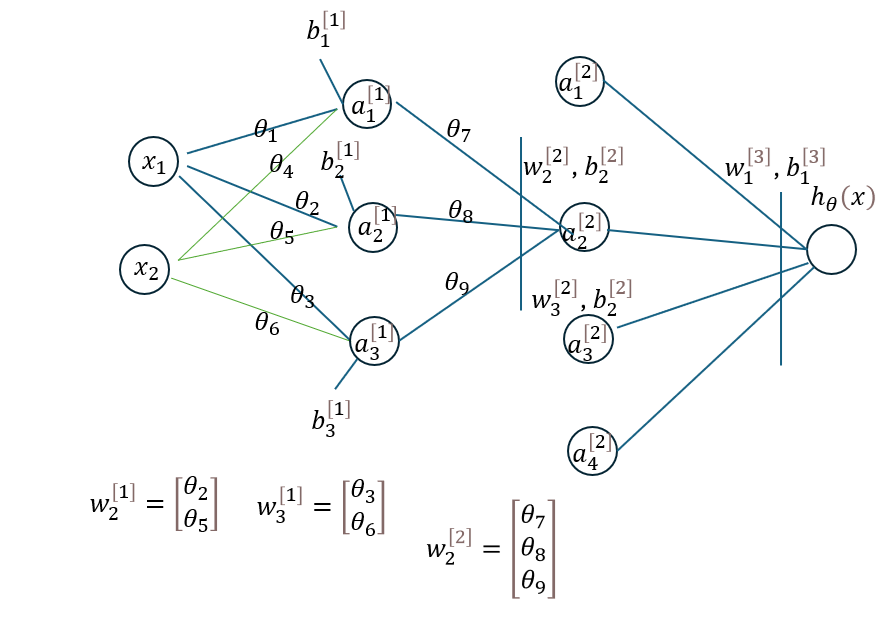
\includegraphics{diagram1}
w's and b's are parameters : Totally ther are Hidden Layer 1 (layer 1) (2x3 + 3) + Hidden Layer 1  (layer 2 ) (3x4 + 4) + Output Layer (layer 3)(4x1 +1 ) number of parameters    
\section{Forward Feed (see above NN diagram) }
\[a_1 = \text{ReLU}(\theta_1 x_1 + \theta_4 x_2 + b_{1}^{[1]})\]
\[a_2 = \text{ReLU}(\theta_2 x_1 + \theta_5 x_2 + b_{2}^{[1]})\]
Let i be \(i^{th}\) layer and j be \(j^{th}\) neuron ( count vertifically) this layer of NN \newline 
Rewriting the notation : \(w_{j}^{[i]}\) as \(\textbf{VECTOR}\) of input \(\theta\)'s for layer i and \(j^{th}\) neuron. \newline
With the above, Layer 1 of NN can be expressed as: \newline 

For all \( j \in [1, \dots, m] \): (m=3, count vertically, is the number of number of neuron layer 1 )
\[
z_j = \mathbf{w}^{[1]}_j{}^\top \mathbf{x} + b^{[1]}_j \quad \text{where} \quad \mathbf{w}^{[1]}_j \in R^d, \; b^{[1]}_j \in R
\]
(d = 2 , count vertically, is the number of number of previous layer , layer 0 )
\[
a_j = \text{ReLU}(z_j),
\]

\[
\mathbf{a} = [a_1, \dots, a_m]^\top \in R^m
\]
For Layer 3 :
\[
\bar{h}_\theta(\mathbf{x}) = \mathbf{w}^{[3]}{}^\top \mathbf{a} + b^{[3]} \quad \text{where} \quad \mathbf{w}^{[3]} \in R^n, \; b^{[3]} \in R
\] 
(n = 4, count vertically, is the number of number of neuron  layer, layer 2  )
\section{Vectorization of Forward Feeding}

Just by stacking the parameters . for layer 1 : 
\[W^{[1]} = \begin{bmatrix} - w^{[1]T}_1 - \\ - w^{[1]T}_2 - \\ \vdots \\ - w^{[1]T}_m - \end{bmatrix} \in R^{m \times d}\]

\[
\mathbf{z} = \begin{bmatrix}
z_1 \\
z_2 \\
\vdots \\
z_m
\end{bmatrix} \in \mathbb{R}^{m \times 1} =
\begin{bmatrix}
-w^{[1]T}_1- \\
-w^{[1]T}_2- \\
\vdots \\
-w^{[1]T}_m-
\end{bmatrix}
\begin{bmatrix}
x_1 \\
x_2 \\
\vdots \\
x_d
\end{bmatrix}
+
\begin{bmatrix}
b^{[1]}_1 \\
b^{[1]}_2 \\
\vdots \\
b^{[1]}_m
\end{bmatrix}
\]
Hence we get: 
\[ z^{[1]}=W^{[1]}x+b^{[1]} \]
\[ a^{[1]} = ReLU(z^{[1]}) \]
\[ z^{[2]}=W^{[2]}a^{[1]}+b^{[2]} \]
\[ a^{[2]} = ReLU(z^{[2]}) \]
\[ h=W^{[3]}a^{[2]}+b^{[3]} \]
In General : 

\[
\begin{aligned}
a^{[1]} &= \text{ReLU}(W^{[1]}x + b^{[1]}) \\
a^{[2]} &= \text{ReLU}(W^{[2]}a^{[1]} + b^{[2]}) \\
&\ \, \vdots \\
a^{[r-1]} &= \text{ReLU}(W^{[r-1]}a^{[r-2]} + b^{[r-1]}) \\
h(x) &= W^{[r]}a^{[r-1]} + b^{[r]}
\end{aligned}
\]
Also, for loss function J
\[J = (1/2)(h-o)^2\]
Some common loss function for J : Common : (1) Mean Sequared Error (2) Cross Entropy Loss 


\section{Vector/Matrix Calculus: Some important equations}
1. Gradient, where f is \(R^n to R\) : \newline

 \( \nabla f(\left.x_{1}, x_{2}, \ldots, x_{n}\right)=\left[\begin{array}{c}
\dfrac{\partial f}{\partial x_1}(\left.x_{1}, x_{2}, \ldots, x_{n}\right)\\
\dfrac{\partial f}{\partial x_2}(\left.x_{1}, x_{2}, \ldots, x_{n}\right) \\
\vdots \\
\dfrac{\partial f}{\partial x_n}(\left.x_{1}, x_{2}, \ldots, x_{n}\right) 
\end{array}\right]\) \newline
Example : \(f(x_1,x_2) = 3x_1^2x_2\), then \( \nabla f(x_1,x_2) = [6x_1x_2,3x_1]^T \) \newline

2. Jacobian of f, Note that there are m DIFFERENT functions 

$$
\begin{aligned}
\mathbf{f}(\mathbf{x})&=\mathbf{f}(x_1,x_2,\dots,x_n)\\
&=(f_1(x_1,x_2,\dots,x_n),,\dots,f_m(x_1,x_2,\dots,x_n))\\
&=(f_1(\mathbf{x}),,\dots,f_m(\mathbf{x}))
\end{aligned}
$$

$$
\mathbb{J}=\left[\begin{array}{ccc}
\dfrac{\partial \mathbf{f}(\mathbf{x})}{\partial x_{1}} & \cdots & \dfrac{\partial \mathbf{f}(\mathbf{x})}{\partial x_{n}}
\end{array}\right]=\left[\begin{array}{c}
\nabla^{T} f_{1}(\mathbf{x}) \\
\vdots \\
\nabla^{T} f_{m}(\mathbf{x})
\end{array}\right]=\left[\begin{array}{ccc}
\dfrac{\partial f_{1}(x_1,x_2....,x_n)}{\partial x_{1}} & \cdots & \dfrac{\partial f_{1}(x_1,x_2....,x_n)}{\partial x_{n}} \\
\vdots & \ddots & \vdots \\
\dfrac{\partial f_{m}((x_1,x_2....,x_n)}{\partial x_{1}} & \cdots & \dfrac{\partial f_{m}((x_1,x_2....,x_n)}{\partial x_{n}}
\end{array}\right]
$$

3. (Law of total derivatives) for \( f(g_1,g_2...., g_k) \) , if  \(\mathbf{EACH}\) of \( g_1,g_2...., g_k \) actually depends on \(x_1,x_2....x_n\), then 
\[
	\dfrac{\partial f_{m}((g_1,g_2....,g_n)}{\partial x_1} = \dfrac{\partial f}{\partial g_1}
\dfrac{\partial g_1}{\partial x_1} + \dfrac{\partial f}{\partial g_2}
\dfrac{\partial g_2}{\partial x_1} + .... + \dfrac{\partial f}{\partial u_n}
\dfrac{\partial g_n}{\partial x_1}
\]
\[
	\dfrac{\partial f_{m}((g_1,g_2....,g_n)}{\partial x_2} = \dfrac{\partial f}{\partial g_1}
\dfrac{\partial g_1}{\partial x_2} + \dfrac{\partial f}{\partial g_2}
\dfrac{\partial g_2}{\partial x_2} + .... + \dfrac{\partial f}{\partial u_n}
\dfrac{\partial g_n}{\partial x_2}
\]
4. By 3 , Jacobian again, but this time : \newline 
\[y_1=f_1(g_1(x_1,...,x_n),g_2(x_1,...,x_n),...,g_k(x_1,...,x_n))\]
\[y_2=f_1(g_1(x_1,...,x_n),g_2(x_1,...,x_n),...,g_k(x_1,...,x_n))\]
\[....\]
\[y_m=f_m(g_1(x_1,...,x_n),g_2(x_1,...,x_n),...,g_k(x_1,...,x_n))\]
\[\mathbf{y} =(y_1,y_2...,y_m) ,  \mathbf{x} = (x_1,...,x_n) \]
\[J=\dfrac{\partial \mathbf{y}}{\partial \mathbf{x}} = \left[\begin{array}{c}
\nabla^{T} f_{1}(\mathbf{x}) \\
\nabla^{T} f_{2}(\mathbf{x}) \\
\vdots \\
\nabla^{T} f_{m}(\mathbf{x})
\end{array}\right]
\]

\[
=\begin{bmatrix}
 \dfrac{\partial f_1}{\partial x_1} & \dfrac{\partial f_1}{\partial x_2} & \cdots & \dfrac{\partial f_1}{\partial x_n} \\ 
 \dfrac{\partial f_2}{\partial x_1} & \dfrac{\partial f_2}{\partial x_2} & \cdots & \dfrac{\partial f_2}{\partial x_n} \\ 
 \cdots & \cdots & \cdots & \cdots \\ 
 \dfrac{\partial f_m}{\partial x_1} & \dfrac{\partial f_m}{\partial x_2} & \cdots & \dfrac{\partial f_m}{\partial x_n}
\end{bmatrix}
\]

\[
=\begin{bmatrix}
 \sum_{i=1}^k \dfrac{\partial f_1}{\partial g_i} \dfrac{\partial g_i}{\partial x_1} & \sum_{i=1}^k \dfrac{\partial f_1}{\partial g_i} \dfrac{\partial g_i}{\partial x_2} & \cdots & \sum_{i=1}^k \dfrac{\partial f_1}{\partial g_i} \dfrac{\partial g_i}{\partial x_2} \\ 
 \sum_{i=1}^k \dfrac{\partial f_2}{\partial g_i} \dfrac{\partial g_i}{\partial x_1} & \sum_{i=1}^k \dfrac{\partial f_2}{\partial g_i} \dfrac{\partial g_i}{\partial x_2} & \cdots & \sum_{i=1}^k \dfrac{\partial f_2}{\partial g_i} \dfrac{\partial g_i}{\partial x_2} \\ 
 \cdots & \cdots & \cdots & \cdots \\ 
 \sum_{i=1}^k \dfrac{\partial f_m}{\partial g_i} \dfrac{\partial g_i}{\partial x_1} & \sum_{i=1}^k \dfrac{\partial f_m}{\partial g_i} \dfrac{\partial g_i}{\partial x_2} & \cdots & \sum_{i=1}^k \dfrac{\partial f_m}{\partial g_i} \dfrac{\partial g_i}{\partial x_2}
\end{bmatrix}
\]
\[
=\begin{bmatrix}
 \dfrac{\partial f_1}{\partial g_1} & \dfrac{\partial f_1}{\partial g_2} & \cdots & \dfrac{\partial f_1}{\partial g_k} \\ 
 \cdots & \cdots & \cdots & \cdots \\ 
 \dfrac{\partial f_m}{\partial g_1} & \dfrac{\partial f_m}{\partial g_2} & \cdots & \dfrac{\partial f_m}{\partial g_k}
\end{bmatrix}
\begin{bmatrix}
 \dfrac{\partial g_1}{\partial x_1} & \dfrac{\partial g_1}{\partial x_2} & \cdots & \dfrac{\partial g_1}{\partial x_n} \\ 
 \cdots & \cdots & \cdots & \cdots \\ 
 \dfrac{\partial g_k}{\partial x_1} & \dfrac{\partial g_k}{\partial x_2} & \cdots & \dfrac{\partial g_k}{\partial x_n}
\end{bmatrix}
\]

5. Jacobian of elementwise operation fuunction are diagonal. Therefore  \( \frac{\partial a^{[i]} }{\partial z^{[i]}} \) is a diagonal matrix \newline

\section{Neural Network breakdown}
\[
z_1^{[1]}=
\begin{bmatrix}
w_{1,1}^{[1]},w_{1,2}^{[1]}
\end{bmatrix}
\begin{bmatrix}
x_1 \\ x_2
\end{bmatrix}
+ b_1^{[1]}
\]

\[
z_2^{[1]}=
\begin{bmatrix}
w_{2,1}^{[1]},w_{2,2}^{[1]}
\end{bmatrix}
\begin{bmatrix}
x_1 \\ x_2
\end{bmatrix}
+ b_2^{[1]}
\]

\[
z_3^{[1]}=
\begin{bmatrix}
w_{3,1}^{[1]},w_{3,2}^{[1]}
\end{bmatrix}
\begin{bmatrix}
x_1 \\ x_2
\end{bmatrix}
+ b_3^{[1]}
\]

\[ a_1^{[1]} = ReLU( z_1^{[1]}), a_2^{[1]} = ReLU( z_2^{[1]}), a_3^{[1]} = ReLU( z_3^{[1]}) \]

\[a^{[1]} = ReLU 
\begin{bmatrix}
\begin{bmatrix}
w_{1,1}^{[1]},w_{1,2}^{[1]} \\ 
w_{2,1}^{[1]},w_{2,2}^{[1]} \\ 
w_{3,1}^{[1]},w_{3,2}^{[1]} 
\end{bmatrix}
\begin{bmatrix}
x_1 \\ x_2
\end{bmatrix} +
\begin{bmatrix}
b_1^{[1]} \\ b_2^{[1]} \\ b_3^{[1]}
\end{bmatrix} 
\end{bmatrix}
\]


\[
z_1^{[2]}=
\begin{bmatrix}
w_{1,1}^{[2]},w_{1,2}^{[2]},w_{1,3}^{[2]}
\end{bmatrix}
\begin{bmatrix}
a_1^{[1]} \\ a_2^{[1]} \\ a_3^{[1]}
\end{bmatrix}
+ b_1^{[2]}
\]

\[
z_2^{[2]}=
\begin{bmatrix}
w_{2,1}^{[2]},w_{2,2}^{[2]},w_{2,3}^{[2]}
\end{bmatrix}
\begin{bmatrix}
a_1^{[1]} \\ a_2^{[1]} \\ a_3^{[1]}
\end{bmatrix}
+ b_2^{[2]}
\]

\[
z_3^{[2]}=
\begin{bmatrix}
w_{3,1}^{[2]},w_{3,2}^{[2]},w_{3,3}^{[2]}
\end{bmatrix}
\begin{bmatrix}
a_1^{[1]} \\ a_2^{[1]} \\ a_3^{[1]}
\end{bmatrix}
+ b_3^{[2]}
\]


\[
z_4^{[2]}=
\begin{bmatrix}
w_{4,1}^{[2]},w_{4,2}^{[2]},w_{4,3}^{[2]}
\end{bmatrix}
\begin{bmatrix}
a_1^{[1]} \\ a_2^{[1]} \\ a_3^{[1]}
\end{bmatrix}
+ b_4^{[2]}
\]

\[ a_1^{[2]} = ReLU( z_1^{[2]}), a_2^{[2]} = ReLU( z_2^{[2]}), a_3^{[2]} = ReLU( z_3^{[2]}), a_4^{[2]} = ReLU( z_4^{[2]}) \]


\[a^{[2]} = ReLU 
\begin{bmatrix}
\begin{bmatrix}
w_{1,1}^{[2]},w_{1,2}^{[2]},w_{1,3}^{[2]} \\ 
w_{2,1}^{[2]},w_{2,2}^{[2]},w_{2,3}^{[2]} \\ 
w_{3,1}^{[2]},w_{3,2}^{[2]},w_{3,3}^{[2]} \\
w_{4,1}^{[2]},w_{4,2}^{[2]},w_{4,3}^{[2]}
\end{bmatrix}
\begin{bmatrix}
a_1^{[1]} \\ a_2^{[1]} \\ a_3^{[1]}
\end{bmatrix} +
\begin{bmatrix}
b_1^{[1]} \\ b_2^{[1]} \\ b_3^{[1]} \\ b_4^{[1]}
\end{bmatrix} 
\end{bmatrix}
\]



\[
z_1^{[3]}=
\begin{bmatrix}
w_{4,1}^{[2]},w_{4,2}^{[2]},w_{4,3}^{[2]},w_{4,4}^{[2]}
\end{bmatrix}
\begin{bmatrix}
a_1^{[1]} \\ a_2^{[1]} \\ a_3^{[1]} \\ a_4^{[1]}
\end{bmatrix}
+ b_1^{[3]}
\]

\[ o = a_1^{[3]} = ReLU( z_1^{[3]}) \]

\[a^{[3]} = ReLU 
\begin{bmatrix}
\begin{bmatrix}
w_{1,1}^{[3]},w_{1,2}^{[3]},w_{1,3}^{[3]},w_{1,3}^{[3]}
\end{bmatrix}
\begin{bmatrix}
a_1^{[2]} \\ a_2^{[2]} \\ a_3^{[2]} \\ a_4^{[2]}
\end{bmatrix} +
\begin{bmatrix}
b_1^{[1]} \\ b_2^{[1]} \\ b_3^{[1]} \\ b_4^{[1]}
\end{bmatrix} 
\end{bmatrix}
\]




\section{Vectorized Backpropagation. (Refer to Section 7)}
Our objective is to make use of matrix calculus, gradient descent to tune W and b to minimize J by SGD or mini-batch GD \newline

Algo 1 SGD : 
 1: Hyperparameter: learning rate \(\alpha\), number of total iteration \(n_{iter}\). \newline
 2: Initialize \(\theta\) randomly. \newline
 3: for i = 1 to niter do \newline
 4: Sample j uniformly from {1,...,n}, and update \(\theta\) by \newline
\[ \theta := \theta - \alpha \nabla_\theta J^{(j)}(\theta) \] 
By Chain Rule of matrix calculus 
\[
\frac{\partial L }{\partial W_{ij}^{[2]}} = ( \frac{\partial L }{\partial a^{[3]}} \frac{\partial a^{[3]}}{\partial z^{[3]}} )
(\frac{\partial z^{[3]}}{\partial a^{[2]}}) ( \frac{\partial a^{[2]}}{\partial z^{[2]}})( \frac{\partial z^{[2]}}{\partial W_{ij}^{[2]}})
\]

\[
= [ (a^{[3]}-y)W[3] \bigodot g(z^{[2]}) ]_i a_j^{[1]T} 
\]
stacking up again :
\[
\frac{\partial L }{\partial W^{[2]}} = [ (a^{[3]}-y)W[3] \bigodot g(z^{[2]}) ] a^{[1]T} 
\]
But How ? Let's do it one-by-one:\newline 

(i) Assume using sigmoid, by differentiation rule : \newline
\[ \frac{\partial L }{\partial z^{[3]}} = \frac{\partial [-ylog(o)-(1-y)(log(1-o))] }{\partial z^{[3]}} = a^{[3]}-y ,\]
 dimension :   \( \epsilon R^{1x1} \)  \newline \newline

(ii) for \( \frac{\partial z^{[3]} }{\partial a^{[2]}} \) \newline
\[ 
\frac{\partial z^{[3]} }{\partial a^{[2]}} = 
\frac{\partial (w_{1,1}^{[3]}a_1^{[2]}+w_{1,2}^{[3]}a_2^{[2]}+w_{1,3}^{[3]}a_3^{[2]}+w_{1,4}^{[3]}a_4^{[2]}) }
{\partial (a_1^{[2]},a_2^{[2]},a_3^{[2]},a_4^{[2]})}
\]
\[ 
= (w_{1,1}^{[3]},w_{1,2}^{[3]},w_{1,3}^{[3]},w_{1,4}^{[3]}) = W^{[3]}
\]
dimension :   \( \epsilon R^{1x4} \)  \newline \newline

(ii) for \( \frac{\partial a^{[2]} }{\partial z^{[2]}} \) \newline
\[ 
\frac{\partial a^{[2]} }{\partial z^{[2]}} = 
\frac{\partial (a_1^{[2]},a_2^{[2]},a_3^{[2]},a_4^{[2]}) }
{\partial (z_1^{[2]},z_2^{[2]},z_3^{[2]},z_4^{[2]})}
\]
\[
=\begin{bmatrix}
 \dfrac{\partial g(z_1^{[2]})}{\partial z_1^{[2]}} & \dfrac{\partial g(z_1^{[2]})}{\partial z_2^{[2]}} & \dfrac{\partial g(z_1^{[2]})}{\partial z_3^{[2]}} & \dfrac{\partial g(z_1^{[2]})}{\partial z_4^{[2]}} \\ 
 \dfrac{\partial g(z_2^{[2]})}{\partial z_1^{[2]}} & \dfrac{\partial g(z_2^{[2]})}{\partial z_2^{[2]}} & \dfrac{\partial g(z_2^{[2]})}{\partial z_3^{[2]}} & \dfrac{\partial g(z_2^{[2]})}{\partial z_4^{[2]}} \\ 
 \dfrac{\partial g(z_3^{[2]})}{\partial z_1^{[2]}} & \dfrac{\partial g(z_3^{[2]})}{\partial z_2^{[2]}} & \dfrac{\partial g(z_3^{[2]})}{\partial z_3^{[2]}} & \dfrac{\partial g(z_3^{[2]})}{\partial z_4^{[2]}} \\ 
 \dfrac{\partial g(z_4^{[2]})}{\partial z_1^{[2]}} & \dfrac{\partial g(z_4^{[2]})}{\partial z_2^{[2]}} & \dfrac{\partial g(z_4^{[2]})}{\partial z_3^{[2]}} & \dfrac{\partial g(z_4^{[2]})}{\partial z_4^{[2]}}
\end{bmatrix}
\]
\[
=\begin{bmatrix}
 g'(z_1^{[2]}) & 0 & 0 & 0  \\ 
 0 & g'(z_2^{[2]}) & 0 & 0 \\ 
0 & 0 &  g'(z_3^{[2]}) &0 \\ 
 0 & 0 & 0 & g'(z_4^{[2]})
\end{bmatrix} = diag(g'(z^{[2]}))
\]
dimension :   \( \epsilon R^{4x4} \)  \newline \newline

(iii) for \( \frac{\partial z^{[2]} }{\partial W_{i,j}^{[2]}} \) \newline
\[
\frac{\partial z^{[2]} }{\partial W_{i,j}^{[2]}}
=\frac{ \partial \begin{bmatrix}
w_{1,1}^{[2]}a_1^{[1]}+w_{1,2}^{[2]}a_2^{[1]}+w_{1,3}^{[2]}a_3^{[1]}+w_{1,4}^{[2]}a_4^{[1]} + b_1^{[1]}\\
w_{2,1}^{[2]}a_1^{[1]}+w_{2,2}^{[2]}a_2^{[1]}+w_{2,3}^{[2]}a_3^{[1]}+w_{2,4}^{[2]}a_4^{[1]} + b_2^{[1]}\\
w_{3,1}^{[2]}a_1^{[1]}+w_{3,2}^{[2]}a_2^{[1]}+w_{3,3}^{[2]}a_3^{[1]}+w_{3,4}^{[2]}a_4^{[1]} + b_3^{[1]}\\
w_{4,1}^{[2]}a_1^{[1]}+w_{4,2}^{[2]}a_2^{[1]}+w_{4,3}^{[2]}a_3^{[1]}+w_{4,4}^{[2]}a_4^{[1]} + b_4^{[1]}
\end{bmatrix} } {\partial W_{i,j}^{[2]}} 
\]
\[
= a_j^{[i]}e_i
\]
for example , if i = 2 , j = 3 : then it is \(a_3 (0,1,0,0)^T=(0,a_3,0,0)^T\) \newline
for example , if i = 4 , j = 4 : then it is \(a_4 (0,0,0,1)^T=(0,0,0,a_4)^T\) \newline
dimension :   \( \epsilon R^{4x1} \)  \newline \newline
We see here the step of GD is based on next layer's value, therefore we have update back propagated to previous layer.
\section{Testing}
\[
\sum_{i=1}^k \frac{\partial f_i}{\partial x_i} dx_i
\]

\end{document}
